\chapter{Kako složiti genomsku slagalicu od milion delova?}
\setbookcodestyle

U ovom poglavlju predstavi\'cemo dati problem i prikazati kako mo\v zemo primeniti grafovske algoritme nad problemom slaganja genomske slagalice. Poglavlje \'cemo zapo\v ceti pri\v com o sekvenciranju genoma. Do sada smo videli \v sta za nas zna\v ci pojam DNK -- da se podsetimo, to je niska karaktera nad azbukom $\Sigma = \{A, C, G, T\}$. Biolo\v ski posmatrano, DNK je molekul koji se nalazi u svakoj \'celiji svakog organizma i da je u njemu zapisan na\v cin pravilnog razvoja i funkcionisanja svakog organizma. 

\section{Šta je sekvenciranje genoma?}

Sa biološke strane, genom jednog organizma predstavlja njegov genetski materijal. Pod genetskim materijalom podrazumevamo delove genoma koji se nasle\dj uju koji se nasle\dj uje i koji svi predstavnici jedne vrste dele u velikoj meri. Kod većine organizama, genetski materijal je sadržan u DNK, odnosno, genom je ekvivalentan sa DNK molekulima. Kod nekih drugih organizama koji su u manjini, kao \v sto su, na primer, virusi, va\v zi da oni ne sadr\v ze DNK i njihov genetski materijal se nalazi u ribonukleinskoj kiselini -- RNK -- o kojoj \'ce biti re\v ci u nastavku. 

Kod čoveka, genom sadrži oko tri milijarde nukleotida. Dakle, sa računarske strane posmatrano genom je niska karaktera nad azbukom $\Sigma = \{A, C, G, T\}$. Kompleksnost organizma nije u relaciji sa veli\v cinom genoma. Genomi nekih organizama su i stotinu puta veći od humanog genoma. Na primer, jedna vrsta amebe ima 670 milijardi nukleotida ili jedna vrsta kaktusa koja raste u Japanu ima 150 milijardi nukleotida.

Sekvenciranje genoma podrazumeva otkrivanje sastava genoma. U pitanju je eksperimentalan proces -- da bismo saznali \v sta se nalazi u sastavu jednog genoma, potreban nam je uzorak tkiva odgovaraju\'ce vrste. U nastavku dajemo kratak pregled razvoja sekvenciranja genoma.

\subsection{Kratka istorija sekvenciranja genoma}

Kao \v sto smo videli, sekvenciranje genoma je eksperimentalan proces, za koji je neophodna veoma sofisticirana tehnologija. Pre svega mo\v zemo govoriti o razvoju fizi\v cko-hemijskih tehnika koje bi dovele do mogu\'cnosti saznavanja sastava genoma. Walter Gilbert i Frederick Sanger su 1977. godine razvili nezavisne metode sa sekvenciranje genoma, za koje su, 1980. godine, podelili Nobelovu nagradu. Me\dj utim, iako su njihovi metodi bili pionirski u ovoj oblasti, njihove metode za sekvenciranje su bile veoma skupe -- za sekvenciranje humanog genoma je bilo potrebno 3 milijarde dolara.

Krajem 2000-ih Sanger metodom je sekvencioniran veliki broj genoma. Visoka cena je bila ograničavajući faktor i za dalji napredak je bila neophodna nova tehnologija sekvencioniranja. \emph{NGS} (skr. \emph{Next Generation Sequencing}) predstavlja metode nove generacije sekvencioniranja, odnosno, novu generaciju ma\v sina sekvencera koji vr\v se sekvencioniranje. \emph{Illumina}, jedan od proizvo\dj a\v ca sekvencera, smanjuje trošak sekvencioniranja humanog genoma sa 3 milijarde na 10 hiljada dolara. Kompanija \emph{Complete Genomics} otvara genomsku fabriku u Silikonskoj dolini koja sekvencionira stotine genoma mesečno. Pekinški genomski institut (\emph{Beijing Genome Institute}, skr. \emph{BGI}) preuzima Complete Genomics 2013. godine i postaje najveći svetski centar za sekvenciranje genoma. Na slici \ref{slika:cena} prikazano je kako se cena sekvencioniranja menjala godinama.

\begin{figure}[h]
	\centering
	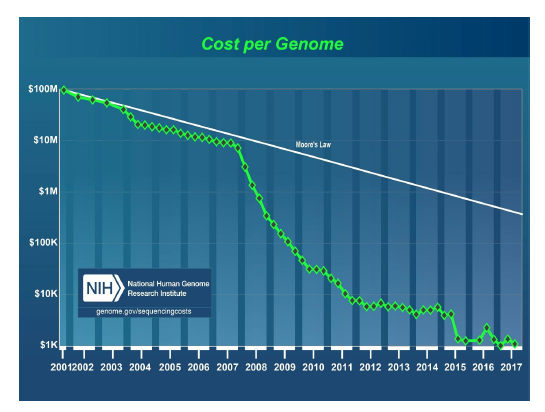
\includegraphics[width=0.95\textwidth]{poglavlja/3/slike/cena_sekvencioniranja.png}
	\caption{Cena sekvencioniranja kroz istoriju.}
	\label{slika:cena}
\end{figure} 

\subsection{Sekvenciranje ličnih genoma}

Prirodno je zapitati se o značaju poznavanja sastava genoma. \v Sto je ti\v ce biljaka, neke od primena sekvenciranja su: razvoj novih biljnih vrsta u poljoprivredi, odre\dj ivanje pogodnog podneblja za neku biljnu vrstu, u farmaciji, i dr. Me\dj utim, najzna\v cajnija primena je u sekvenciranju li\v cnih genoma.

Genomi se kod različitih ljudi razlikuju na malom broju pozicija (u proseku sadrže jednu mutaciju na hiljadu nukleotida). Ova razlika je odgovorna za, na primer, različite visine kod ljudi, da li će imati sklonost ka visokom holesterolu ili ne, za veliki broj genetskih bolesti, itd.

Godine 2010. Nicholas Volker je postao prvo ljudsko biće čiji je život spašen zahvaljujući genomskom sekvencioniranju. Lekari nisu mogli da postave tačnu dijagnozu i morali su da ga podvrgnu velikom broju operacija pokušavajući da je utvrde. Sekvenciranje je otkrilo retku mutaciju na jednom genu (XIAP) koja je bila povezana sa oštećenjem njegovog imunog sistema. Ovo otkriće je navelo lekare na adekvatnu terapiju koja je rešila problem.

\section{Eksplozija u štampariji}

Razmotrimo slede\'ci primer. Neka imamo hiljadu kopija istog izdanja novina na jednoj gomili, a ispod njih postavljen je dinamit. Upalimo fitilj i zamislimo da nije sve samo izgorelo već da se raspršilo u milione delića papira. Kako možemo da iskoristimo te deliće da bismo saznali koje su bile vesti iz tog izdanja? Ovaj problem nazvaćemo \emph{Problem novina} (videti sliku \ref{slika:eksplozija}). 

\begin{figure}[h]
	\centering
	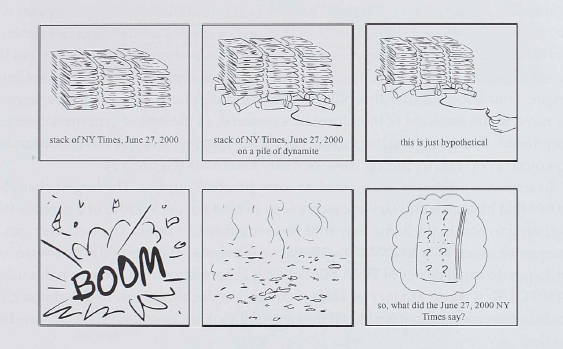
\includegraphics[width=1\textwidth]{poglavlja/3/slike/eksplozija.png}
	\caption{Problem novina poslužiće nam u razumevanju problema slaganja genoma.}
	\label{slika:eksplozija}
\end{figure} 

Problem novina je mnogo teži nego što izgleda. Kako smo imali više kopija istog izdanja, i kako smo izgubili neki deo informacija prilikom eksplozije, ne možemo samo da prilepimo deliće novina kao da su slagalica. Umesto toga, potrebno je da preklopimo delove različitih novina kako bismo rekonstruisali jedan primerak.

\begin{figure}[h]
	\centering
	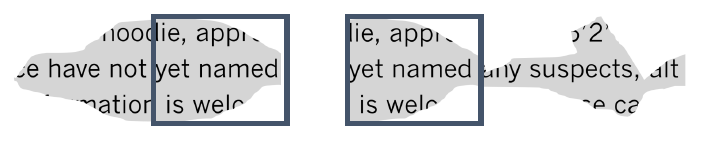
\includegraphics[width=1\textwidth]{poglavlja/3/slike/delici.png}
	\caption{Spajanje delova različitih novina koji se jednim delom preklapaju.}
	\label{slika:delici}
\end{figure} 

Određivanje redosleda nukleotida u genomu, odnosno sekvenciranje genoma, predstavlja bitan problem u bioinformatici. Ve\'c smo pomenuli da dužine genoma variraju -- humani genom je dugačak oko 3 milijarde nukleotida, dok je genom jednoćelijskog organizma \emph{Amoeba dubia} čak 200 puta duži. 

Razmotrimo sada povezanost problema novina i sekvenciranja genoma. Kopije izdanja u problemu novina odgovaraju ono predstavlja ulaz u sekvencerima -- uzorak tkiva. Moderne mašine za sekvenciranje ne mogu da pročitaju ceo genom nukleotid po nukleotid od početka do kraja (kao što bismo pročitali knjigu). Mogu samo da iseckaju genom i generišu njegova kratka \emph{očitavanja} (engl. \emph{reads}). Kako to zapravo funkcioniše? 

Na slici \ref{slika:sekvenciranje} ilustrovan je proces sekvenciranja. Sekvencer dobija milione kopija istog genoma. Zatim vrši očitavanja čime dobijamo deliće odnosno kratke podniske. Neki delovi odnosno očitavanja biće izgubljena (kao delići novina u eksploziji, dakle gubimo deo informacija). Očitavanja su izmešana i ono što nam sekvencer daje je zapravo kolekcija podniski koje treba spojiti u jednu. Sastavljanje genoma nije isto kao i slaganje slagalice -- moramo da koristimo preklapajuća očitavanja da bismo rekonstruisali genom.

\begin{figure}[h]
	\centering
	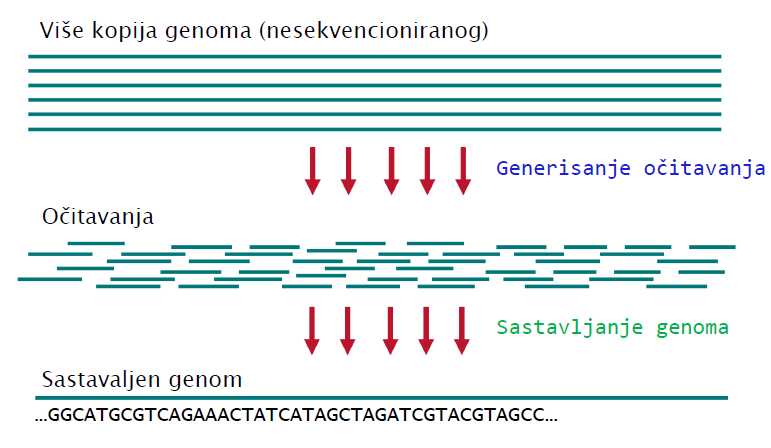
\includegraphics[width=1\textwidth]{poglavlja/3/slike/sekvencioniranje.png}
	\caption{Ilustracija problema.}
	\label{slika:sekvenciranje}
\end{figure} 

\section{Problem sekvenciranja genoma}

Do sada smo videli \v sta predstavlja sekvenciranje genoma, koja je njegova biolo\v ska podloga i kako se on defini\v se kao biolo\v ski problem. Pre\dj imo sada na formulisanje ra\v cunarskog problema sekvenciranja genoma kao problem rekonstrukcije niske.
~ \\
\begin{tcolorbox}
	\textbf{Problem sekvencioniranja genoma:} Rekonstruisati genom na osnovu očitavanja. \\
	\textit{Ulaz:} Kolekcija niski \emph{Reads}.\\
	\textit{Izlaz:} Niska \emph{Genome} rekonstruisana na osnovu \emph{Reads}.
\end{tcolorbox}

~\\
Ovo nije dobro definisan problem. Potrebno je uvesti dodatne pojmove kako bismo uspeli da problem sekvencioniranja genoma predstavimo kao problem rekonstrukcije niske.

Defini\v semo pojam \emph{$k$-gramski sastav niske} na slede\'ci na\v cin. $k$-gramski sastav niske $Text$, u oznaci $Composition_k(Text)$, predstavlja kolekciju podniski dužine $k$ niske $Text$, pri \v cemu su u kolekciju uključeni duplikati. Na primer, neka je $Text=TAATGCCATGGGATGTT$. Njen $3$-gramski sastav niske $Text$ izgleda:

\newpage
\begin{lstlisting}
Composition_3(TAATGCCATGGGATGTT) =
              TAA 
               AAT 
                ATG
                 TGC
                  GCC
                   CCA
                    CAT
                     ATG
                      TGG
                       GGG
                        GGA
                         GAT
                          ATG
                           TGT
                            GTT
\end{lstlisting}

\noindent odnosno, ako kolekciju uredimo po leksikografskom pore\dj enju:

\begin{lstlisting}
Composition_3(TAATGCCATGGGATGTT) =
AAT ATG ATG ATG CAT CCA GAT GCC GGA GGG GTT TAA TGC TGG TGT
\end{lstlisting}

Sada možemo malo bolje da definišemo problem.
~ \\
\begin{tcolorbox}
	\textbf{Problem rekonstrukcije niske:} Rekonstruisati nisku na osnovu njenog $k$-gramskog sastava. \\
	\textit{Ulaz:} Kolekcija $k$-grama.\\
	\textit{Izlaz:} Niska \emph{Genome} takva da je $Composition_k(Genome)$ ekvivalentno kolekciji $k$-grama.
\end{tcolorbox}

~\\

Zapo\v cnimo prvo sa naivnim pristupom re\v savanju ovog problema. Odaberimo jedan $k$-gram za početni. Zatim nižemo ostale tako da se sufiks poslednjeg odabranog poklopi sa prefiksom nekog od preostalih $k$-grama. Pri tome, ako ima više takvih $k$-grama, biramo proizvoljan jedan. Na ovaj način možemo doći do rešenja, ali je veoma skupo. Pri tome, velika je šansa da ćemo se negde zaglaviti (tj. nijedan od preostalih $k$-grama neće biti kandidat za nadovezivanje na tekuću nisku) ili zbog izbora početnog $k$-grama ili zbog izbora nekog od preostalih $k$-grama kada je postojalo više odgovarajućih. Sledeći primer ilustruje ovaj problem.

Neka nam je dat sledeći 3-gramski sastav: \texttt{AAT ATG ATG ATG CAT CCA GAT GCC GGA GGG GTT TAA TGC TGG TGT}. Treba rekonstruisati nisku koja ima takav sastav. Biramo početni 3-gram, neka to bude na primer \texttt{TAA}. Zatim na njega treba nadovezati 3-gram koji počinje njegovim sufiksom dužine 2, odnosno onaj 3-gram koji ima prefiks \texttt{AA}. U našem slučaju, postoji jedan takav 3-gram i njega nadovezujemo na tekuću nisku, tako da sada imamo \texttt{TAAT}. Zatim biramo 3-gram čiji je prefiks \texttt{AT}. Ovog puta imamo 3 kandidata, ali, na našu sreću, sva tri su isti 3-grami, \texttt{ATG}. U takvom slučaju nije bitno koji smo odabrali, jer su svi jednaki. Nadovezujemo ga na tekuću nisku i dobijamo \texttt{TAATG}. Tražimo 3-grame sa prefiksom \texttt{TG}, koji do sad nisu upotrebljeni. Ponovo pronalazimo 3 kandidata. Međutim, u ovom slučaju, svi kandidati predstavljaju različite 3-grame, a to su \texttt{TGC}, \texttt{TGG} i \texttt{TGT}. Naivni pristup kaže da biramo jedan od njih, i recimo da smo odabrali \texttt{TGT} i dobili nisku \texttt{TAATGT}. Sada nam je potreban 3-gram sa prefiksom \texttt{GT} i tu dolazi do zaglavljivanja. Imamo još 3-grama koji nisu iskorišćeni za rekonstrukciju niske, ali nijedan ne možemo da iskoristimo u ovom trenutku. U takvim situacijama treba se vratiti u nazad do koraka u kom je bilo više kandidata.

\section{Rekonstrukcija niske kao problem Hamiltonove putanje}

Videli smo da nam naivni pristup ne odgovara i moramo smisliti bolje rešenje. Mogli bismo da iskoristimo znanja iz teorije grafova za rešavanje ovakvog problema. U tom slučaju, prvi zadatak je da našu nisku predstavimo u vidu grafa.

\subsection{Genom kao putanja}

Vratimo se na prethodni primer. Dat nam je naredni 3-gramski sastav:
\begin{lstlisting}
Composition_3(TAATGCCATGGGATGTT) =
              TAA 
               AAT 
                ATG
                 TGC
                  GCC
                   CCA
                    CAT
                     ATG
                      TGG
                       GGG
                        GGA
                         GAT
                          ATG
                           TGT
                            GTT
\end{lstlisting}

Ovakav 3-gramski sastav mo\v zemo predstaviti kao graf na slede\'ci na\v cin. Svakom \v cvoru u grafu odgovara jedan od $k$-grama. Zatim, potrebne su nam grane koje će povezati te čvorove. Dva čvora su povezana usmerenom granom ako izlazni čvor ima sufiks koji je jednak prefiksu ulaznog čvora te grane, kao što je prikazano na slici \ref{slika:hamilton}.

\begin{figure}[H]
	\centering
	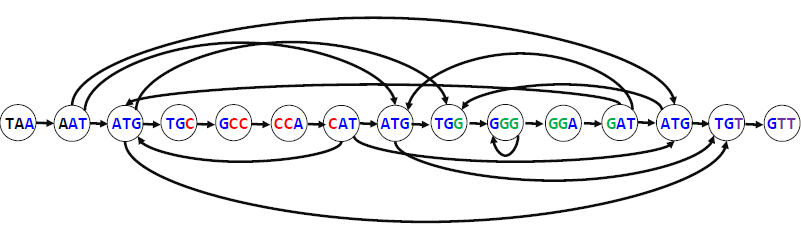
\includegraphics[width=1\textwidth]{poglavlja/3/slike/hamilton.png}
	\caption{Graf koji odgovara 3-gramskom sastavu niske $TAATGCCATGGGATGTT$.}
	\label{slika:hamilton}
\end{figure} 

Jasno je da postoji više puteva u ovom grafu. Postavlja se pitanje -- da li možemo da pronađemo genomsku putanju u ovom grafu, od svih koje postoje?

Podsetimo se šta je Hamiltonova putanja. Hamiltonova putanja je putanja koja posećuje svaki čvor u grafu tačno jednom. To je upravo ono što nam je potrebno za rešavanje problema. Svaki čvor predstavlja jedan $k$-gram i potrebno nam je da svi $k$-grami budu uključeni u rekonstruisanu nisku tačno jednom.
~ \\
\begin{tcolorbox}
	\textbf{Problem Hamiltonove putanje:} Naći Hamiltonovu putanju u grafu. \\
	\textit{Ulaz:} Graf.\\
	\textit{Izlaz:} Putanja koja posećuje svaki čvor u grafu tačno jednom.
\end{tcolorbox}

~\\

Iako deluje kao da smo rešili sve probleme, zapravo smo naišli na još jednu veliku prepreku. Naime, pronalaženje Hamiltonovog puta u grafu je NP-kompletan problem, što znači da ne postoji algoritam koji ga rešava u polinomijalnom vremenu. U tom slučaju, moramo da se vratimo na početak, a to je predstavljanje $k$-gramskog sastava grafom.

\section{Rekonstrukcija niske kao Ojlerove putanje}

U prethodnoj sekciji, $k$-grame smo predstavili čvorovima u grafu i u njemu tražili Hamiltonov put, odnosno, put koji obilazi svaki čvor tačno jednom. Videli smo da za taj problem još uvek nije poznat efikasan algoritam pa se sada pitamo kako možemo izmeniti graf tako da ne zahteva traženje Hamiltonove putanje.

Ono što se javlja kao ideja jeste obeležavanje grana umesto čvorova. Dakle, svaka grana biće obeležena jednim $k$-gramom. Izlazni čvor biće obeležen prefiksom $k$-grama te grane, dok će ulazni čvor biti obeležen sufiksom istog tog $k$-grama. Slika \ref{slika:ojler} ilustruje ovaj postupak za nisku $TAATGCCATGGGATGTT$.

\begin{figure}[h]
	\centering
	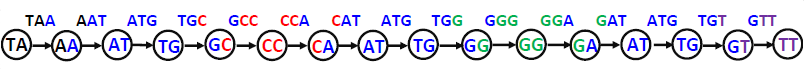
\includegraphics[width=1\textwidth]{poglavlja/3/slike/ojler.png}
	\caption{Graf koji odgovara 3-gramskom sastavu niske $TAATGCCATGGGATGTT$. Grane su obeležene 3-gramima, a čvorovi 2-gramima koji predstavljaju prefikse i sufikse.}
	\label{slika:ojler}
\end{figure} 

Primećujemo da su neki čvorovi obleženi identično (na primer, imamo tri čvora sa oznakom $AT$). Sve čvorove koji imaju istu oznaku treba spojiti u jedan, pri čemu zadržavamo sve grane koje su ulazile u taj čvor ili su izlazile iz njega. Ponavljamo postupak dokle god imamo čvorove koji imaju istu oznaku i na kraju dobijamo graf koji nazivamo \emph{De Brojnov graf}. Slika \ref{slika:debrojnov} ilustruje De Brojnov graf dobijen ovom procedurom od polaznog grafa sa slike \ref{slika:ojler}. 

\begin{figure}[h]
	\centering
	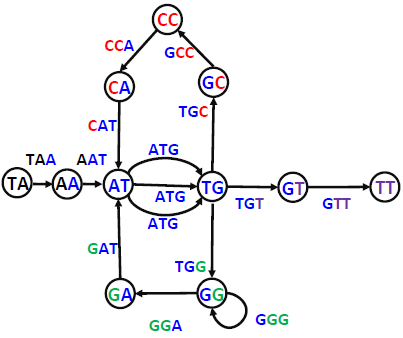
\includegraphics[width=0.55\textwidth]{poglavlja/3/slike/debrojnov.png}
	\caption{De Brojnov graf koji odgovara niski $TAATGCCATGGGATGTT$.}
	\label{slika:debrojnov}
\end{figure} 

Ovime smo dobili novu reprezentaciju niske pomoću grafa. Prirodno se postavlja naredno pitanje -- gde se nalazi niska \textit{Genome} u ovoj reprezentaciji grafa? Kako nam se 3-grami sada nalaze na granama, a ne u čvorovima, potrebno je da pronađemo putanju u grafu koja prolazi sve grane tačno jednom. Takav put nazivamo \emph{Ojlerova putanja}. Srećom, algoritam za pronalaženje Ojlerove putanje u grafu nije NP-kompletan i možemo efikasno da je pronađemo.
~ \\
\begin{tcolorbox}
	\textbf{Problem Ojlerove putanje:} Pronaći Ojlerovu putanju u grafu. \\
	\textit{Ulaz:} Graf.\\
	\textit{Izlaz:} Putanja koja posećuje svaku granu u grafu tačno jednom.
\end{tcolorbox}

~\\

Sada znamo kako možemo da dobijemo nisku kada znamo De Brojnov graf koji odgovara njenom $k$-gramskom sastavu. Međutim, konstruisali smo De Brojnov graf na osnovu genoma, ali u realnim primenama, genom je nepoznat.

\section{De Brojnovi grafovi na osnovu kolekcije $k$-grama}

Videli smo kako mo\v zemo od zadate niske prona\'ci De Brojnov graf. Na\v zalost, u primenama nije nam poznata niska, ali znamo njen $k$-gramski sastav. Postavlja se pitanje kako mo\v zemo konstruisati De Brojnov graf od $k$-gramskog sastava niske. 

Za svaki $k$-gram pravimo dva čvora i jednu granu -- oznaka grane je upravo taj $k$-gram, oznaka izlaznog \v cvora je prefiks, a ulaznog \v cvora je sufiks datog $k$-grama. Time dobijamo nepovezani graf kao na slici \ref{slika:kgrami}. Zatim lepimo identične čvorove sve dok ne dobijemo graf čiji svi čvorovi imaju različite oznake. Na slici \ref{slika:lepljenje} dat je jedan korak ovog postupka, međutim, tu nije kraj jer i dalje postoje čvorovi sa istim oznakama.

\begin{figure}[h]
	\centering
	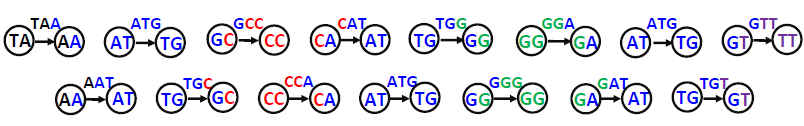
\includegraphics[width=1\textwidth]{poglavlja/3/slike/debrojnov1.png}
	\caption{Svaki k-gram prestavljen je pomoću dva čvora i jedne grane.}
	\label{slika:kgrami}
\end{figure} 

\begin{figure}[h]
	\centering
	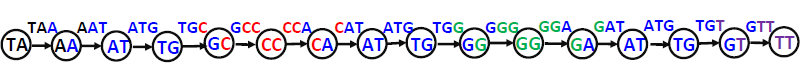
\includegraphics[width=1\textwidth]{poglavlja/3/slike/lepljenje.png}
	\caption{Prvi korak u postupku lepljenja čvorova. Napomenimo da postupak nije završen jer treba zalepiti čvorove sa identičnim oznakama (na primer, AT).}
	\label{slika:lepljenje}
\end{figure} 

Po završetku postupka dobijamo de Brojnov graf koji je isti kao onaj koji smo dobili kada smo znali nisku, odnosno, graf na slici \ref{slika:debrojnov}. Svaka grana je označena jednim $k$-gramom, a svaki čvor je označen prefiksom, odnosno, sufiksom odgovaraju\'ce izlazne, odnosno, ulazne grane, redom. Naravno, \v cvovori koji imaju identi\v cne oznake su zalepljeni.

\section{Ojlerova teorema}

Za re\v savanje problema Ojlerove putanje koji smo predstavili u prethodnoj sekciji mo\v zemo iskoristiti re\v senje narednog problema. Ovaj problem je zna\v cajan jer postoji teorema koja ga prati, a koja odre\dj uje uslove za njegovo re\v savanje.

~ \\
\begin{tcolorbox}
	\textbf{Problem Ojlerovog ciklusa:} Pronaći Ojlerov ciklus u grafu. \\
	\textit{Ulaz:} Graf.\\
	\textit{Izlaz:} Ciklus koji posećuje svaku granu u grafu tačno jednom.
\end{tcolorbox}

~\\


Ka\v zemo da je graf Ojlerov ako sadr\v zi Ojlerov ciklus. Ispostavlja se da postoje odre\dj ene karakteristike koje odre\dj uju da li je graf Ojlerov. Uvedimo pojmove povezan graf i balansiran graf. Kažemo da je graf \emph{povezan} ako za ma koja dva čvora postoji putanja koja ih povezuje. Graf je \emph{balansiran} ako za svaki čvor važi da mu je izlazni stepen jednak ulaznom. Naredna teorema govori o potrebnim i dovoljnim uslovima da graf bude Ojlerov.

\begin{teorema}[Ojlerova teorema]
	Svaki Ojlerov graf je balansiran. Svaki povezan graf i balansiran graf je Ojlerov.
\end{teorema}

\subsection{Dokaz Ojlerove teoreme}

Neka nam je dat povezan balansiran graf. Da bismo pokazali da graf sadrži Ojlerov ciklus, postavićemo mrava na bilo koji od čvorova tog grafa, kao na slici \ref{slika:mrav1}. Zašto baš mrav? Poznato je da mravi nikada ne idu istim putem dva puta pa smo sigurni da će naš mrav proći svaku granu tačno jednom.

Puštamo mrava da slučajno odabira grane kojima će se kretati. Ako je veoma pametan, obići će svaku granu jednom i vratiće se u početni čvor. Međutim, velike su šanse da nije veoma pametan i da će se u nekom čvoru zaglaviti, odnosno, neće imati granu koju već nije obišao.

Da li mrav može da se zaglavi u bilo kom čvoru? Ispostavlja se da može da se zaglavi samo u početnom čvoru (jer je graf balansiran). U trenutku kada se zaglavio on je napravio ciklus. Samo, taj ciklus nije Ojlerov jer još uvek nije obišao sve grane. Ideja je da odabere drugačiji početni čvor iz kog će krenuti obilazak. Koji čvor će izabrati? Treba da izabere čvor iz ciklusa koji ima izlaznih grana koje još uvek nije obišao (slika \ref{slika:mrav2}). 

\noindent
\begin{minipage}{\textwidth}
	\centering
	\begin{minipage}{0.45\textwidth}
		\begin{figure}[H]
			\centering
			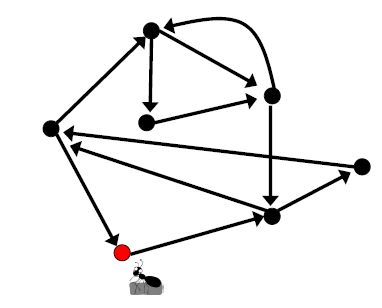
\includegraphics[width=\textwidth]{poglavlja/3/slike/mrav1.png}
			\caption{Mrav je postavljen u crveni čvor i odatle kreće obilazak povezanog balansiranog grafa.}
			\label{slika:mrav1}
		\end{figure} 
	\end{minipage}
	\hfill 
	\begin{minipage}{0.45\textwidth}
		\begin{figure}[H]
			\centering
			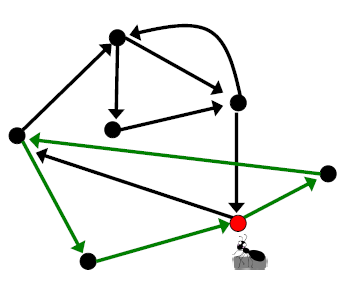
\includegraphics[width=\textwidth]{poglavlja/3/slike/mrav2.png}
			\caption{Mrav se zaglavio i pokušava ponovo iz drugog čvora koji pripada ciklusu i ima izlazne grane koje nisu posećene.}
			\label{slika:mrav2}
		\end{figure} 
	\end{minipage}
	\vspace*{1em}
\end{minipage}

Sada, mrav pokušava ispočetka iz novog čvora. Prvo obilazi ciklus koji je već pronašao u prethodnom pokušaju, a zatim nastavlja obilazak preko neposećenih grana. Na taj način, ciklus se uvećava dok se ne dođe do Ojlerovog. Ukoliko se ponovo zaglavi (slika \ref{slika:mrav3}) ponovo bira novi početni čvor, obilazi pronađeni ciklus (koji i dalje nije Ojlerov) i tako sve dok ne uspe da obiđe sve grane (slika \ref{slika:mrav4}).

\newpage
Dokaz Ojlerove teoreme daje primer konstruktivnog dokaza, koji ne dokazuje samo željeni rezultat, već pruža metod za konstrukciju onoga što nam je potrebno. Ukratko, pratili smo kretanje mrava dok nije pronašao Ojlerov ciklus u povezanom balansiranom grafu, što je sumirano u algoritmu \texttt{EulerianCycle}.

\noindent
\begin{minipage}{\textwidth}
	\centering
	\begin{minipage}{0.45\textwidth}
		\begin{figure}[H]
			\centering
			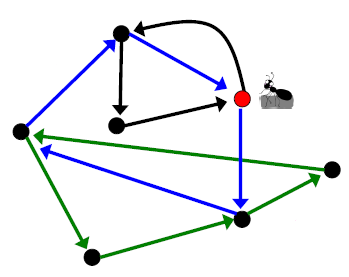
\includegraphics[width=\textwidth]{poglavlja/3/slike/mrav3.png}
			\caption{Mrav se ponovo zaglavio i pokušava od novog čvora.}
			\label{slika:mrav3}
		\end{figure} 
	\end{minipage}
	\hfill 
	\begin{minipage}{0.45\textwidth}
		\begin{figure}[H]
			\centering
			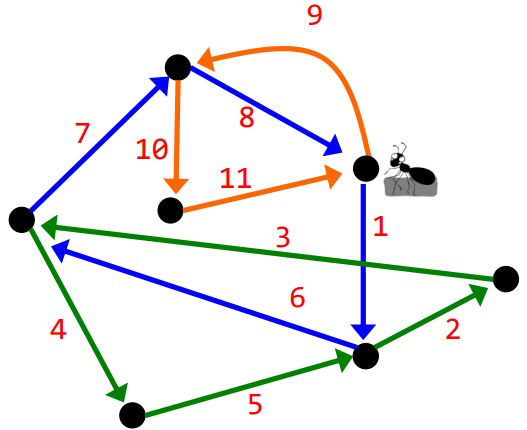
\includegraphics[width=\textwidth]{poglavlja/3/slike/mrav4.png}
			\caption{Mrav je konačno uspeo da pronađe dobar početni čvor i Ojlerov ciklus. Grane su obeležene redosledom kojim su posećene.}
			\label{slika:mrav4}
		\end{figure} 
	\end{minipage}
	\vspace*{1em}
\end{minipage}

\begin{lstlisting}
EulerianCycle(BalancedGraph)
begin
	form a Cycle by randomly walking in BalancedGraph (avoiding already visited edges)
	while Cycle is not Eulerian
		select a node newStart in Cycle with still unexplored outgoing edges
		form a Cycle' by traversing Cycle from newStart and randomly walking afterwards
		Cycle %$\leftarrow$% Cycle'
	return Cycle
end
\end{lstlisting}

Ovaj algoritam radi u linearnom vremenu. Da bi se zaista postigla ta efikasnost, potrebne su efikasne struktutre podataka za održavanje ciklusa koje mrav pronalazi kao i za liste neiskorišćenih grana za svaki čvor i lista čvorova u trenutnom ciklusu koji imaju neiskorišćene grane.

\section{Sastavljanje parova očitavanja}

Predstavimo kao da su svi naši problemi rešeni. Međutim, može se javiti više Ojlerovih putanja u grafu. Srećom, i za ovo imamo jednostavno rešenje.

\subsection{DNK sekvenciranje sa parovima očitavanja} 

Imamo više identičnih kopija genoma i na slučajnim pozicijama sečemo genom na fragmente iste dužine \textit{InsertLength}. Zatim generišemo \emph{parove očitavanja} -- dva očitavanja sa krajeva svakog fragmenta na jednakoj, fiksiranoj udaljenosti. Pod \emph{uparenim $k$-gramom} podrazumevamo par $k$-grama na fiksiranom rastojanju $d$ u genomu. \emph{Upareni $k$-gramski sastav}, u oznaci $PairedComposition_k(Text)$, sastoji se od svih $k$-grama niske $Text$ i njihovih parova.

\begin{figure}[h]
	\centering
	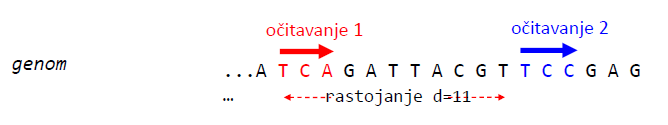
\includegraphics[width=1\textwidth]{poglavlja/3/slike/upareni_kgram.png}
	\caption{\texttt{TCA} i \texttt{TCC} na rastojanju $d=11$ čine jedan upareni 3-gram.}
	\label{slika:upareni}
\end{figure} 

Dajmo jedan primer. Neka imamo nisku \texttt{TAATGCCATGGGATGTT}, i upareni 3-gram \texttt{TAA} i \texttt{GCC}. Upareni $k$-gramski sastav date niske prikazan je na slici \ref{slika:upareni3}.

\begin{figure}[h]
	\centering
	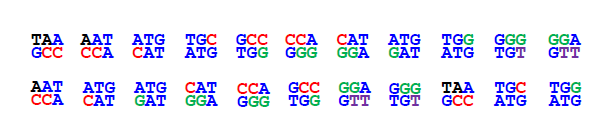
\includegraphics[width=1\textwidth]{poglavlja/3/slike/upareni_3gram.png}
	\caption{\emph{PairedComposition} niske \texttt{TAATGCCATGGGATGTT} i njegov leksikografski poredak.}
	\label{slika:upareni3}
\end{figure} 

Sada mo\v zemo formulisati naredni problem.

~ \\
\begin{tcolorbox}
	\textbf{Problem rekonstrukcije niske na osnovu parova očitavanja:}	Rekonstruisati nisku na osnovu njenih uparenih $k$-grama. \\
	\textit{Ulaz:} Kolekcija uparenih $k$-grama.\\
	\textit{Izlaz:} Niska $Text$ takva da je $PairedComposition_k(Text)$ jednak kolekciji uparenih $k$-grama. 
\end{tcolorbox}

~\\

Kako konstruisati upareni De Brojnov graf na osnovu uparenog $k$-gramskog sastava? Postupak je sličan prethodnom slučaju, kada nismo imali parove. Pretpostavimo da je dat genom (niska $Genome$). Posmatrajmo genom kao putanju u grafu obeleženom na osnovu njegovog uparenog $k$-gramskog sastava (videti sliku \ref{slika:upareniDeBrojnov}). Svaka grana obeležena je uparenim $k$-gramom, a svaki čvor uparenim prefiksom, odnosno, sufiksom $k$-grama.

\begin{figure}[h]
	\centering
	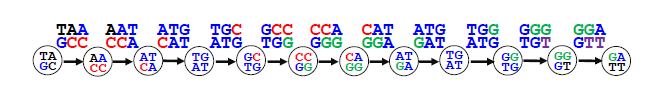
\includegraphics[width=1\textwidth]{poglavlja/3/slike/upareni_debrojnov.png}
	\caption{Graf koji odgovara uparenom 3-gramskom sastavu niske \texttt{TAATGCCATGGGATGTT}.}
	\label{slika:upareniDeBrojnov}
\end{figure} 

Potrebno je zalepiti čvorove sa istom oznakom, tako da svi čvorovi budu jedinstveno obeleženi. Postupak je identičan prethodnom slučaju, odnosno, kada nismo imali parove. Primetimo da sada imamo mnogo manje lepljenja jer imamo samo dva čvora sa istom oznakom (\texttt{TG} \texttt{AT}), (videti sliku \ref{slika:uparenoLepljenje}).

\begin{figure}[h]
	\centering
	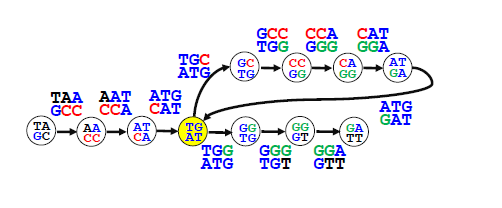
\includegraphics[width=1\textwidth]{poglavlja/3/slike/upareno_lepljenje.png}
	\caption{Dva čvora sa oznakom (\texttt{TG AT}) spajaju se u jedan pri čemu su sve grane, incidentne sa tim čvorovima, očuvane.}
	\label{slika:uparenoLepljenje}
\end{figure} 

Kao i u prethodnom slučaju, pretpostavili smo da je dat genom (niska $Genome$), što često nije slučaj. Posmatrali smo genom kao putanju u grafu obeleženom na osnovu njegovog uparenog $k$-gramskog sastava. Sada pretpostavimo da nije dat genom već samo upareni $k$-gramski sastav. Za svaki upareni $k$-gram pravimo dva čvora i jednu granu, zatim lepimo identične čvorove (videti \ref{slika:uparenoLepljenje2}), i na kraju dobijamo upareni De Brojnov graf, kao onaj na slici \ref{slika:uparenoLepljenje}.

\begin{figure}[h]
	\centering
	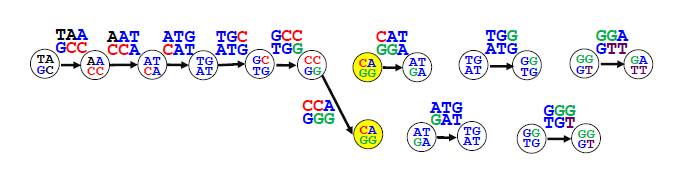
\includegraphics[width=1\textwidth]{poglavlja/3/slike/upareno_lepljenje2.png}
	\caption{Konstrukcija uparenog De Brojnovog grafa na osnovu uparenih $k$-grama.}
	\label{slika:uparenoLepljenje2}
\end{figure} 

Dakle, upareni De Brojnov graf, na osnovu kolekcije uparenih $k$-grama, dobijamo tako što svaku granu označavamo jednim uparenim $k$-gramom. Zatim, svaki čvor označavamo prefiksima, odnosno, sufiksima odgovaraju\'ce izlazne, odnosno, ulazne grane, redom. Na kraju, lepimo čvorove sa identičnim oznakama.

\section{U realnosti}

Ovde smo imali neke nerealne pretpostavke:

\begin{itemize}
	\item Savršena pokrivenost genoma očitavanjima (svaki $k$-gram iz genoma je očitan). Očitavanja dužine 250 nukleotida dobijena \emph{Illumina} tehnologijom predstavljaju samo mali deo 250-grama unutar genoma. Rešenje je u razbijanju dobijenih očitavanja na kraće $k$-grame (kao na slici \ref{slika:manji kgrami}).
	
	\item Očitavanja ne sadrže greške. U ovom slu\v caju, ako bismo razbili na manje $k$-grame, onda bismo dobili vi\v se niski koje imaju pogre\v sno o\v citavanje. Postavljamo pitanje kako se ovakvi slu\v cajevi manifestuju u konstrukciji DeBrojnovog grafa. Dolazi do stvaranja \emph{balon\v ci\'ca} (engl. \emph{bubble}) u grafu (videti sliku \ref{slika:baloncic}). Jednostavan je slu\v caj kada govorimo o gre\v sci na jednom o\v citavanju, me\dj utim, ukoliko postoji vi\v se gre\v saka, onda dolazi do \emph{eksplozije balon\v ci\'ca} (videti sliku \ref{slika:eksplozija baloncica}).
	
	\item Rastojanja između očitavanja u okviru parova očitavanja su egzaktna.
	
	\item itd.
\end{itemize}


\begin{figure}[H]
	\centering
	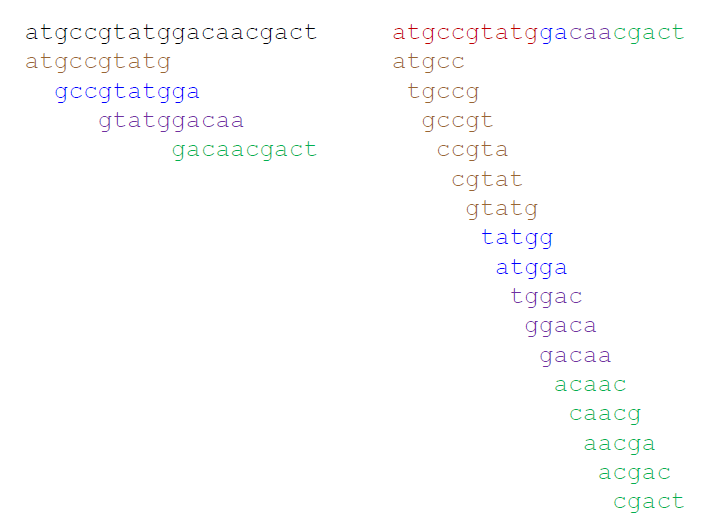
\includegraphics[width=\textwidth]{poglavlja/3/slike/razbijanje_na_manje_kgrame.png}
	\caption{Primer razbijanja dobijenih očitavanja na manje k-grame.}
	\label{slika:manji kgrami}
\end{figure}

\begin{figure}[H]
	\centering
	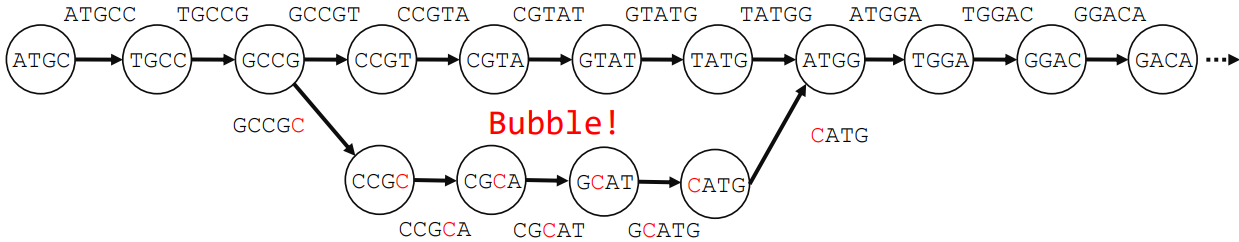
\includegraphics[width=\textwidth]{poglavlja/3/slike/baloncic.png}
	\caption{Primer pojave balon\v ci\'ca u De Brojnovom grafu usled pojave gre\v ske u o\v citavanju nukleotida \texttt{T} nukleotidom \texttt{C}.}
	\label{slika:baloncic}
\end{figure} 

\begin{figure}[H]
	\centering
	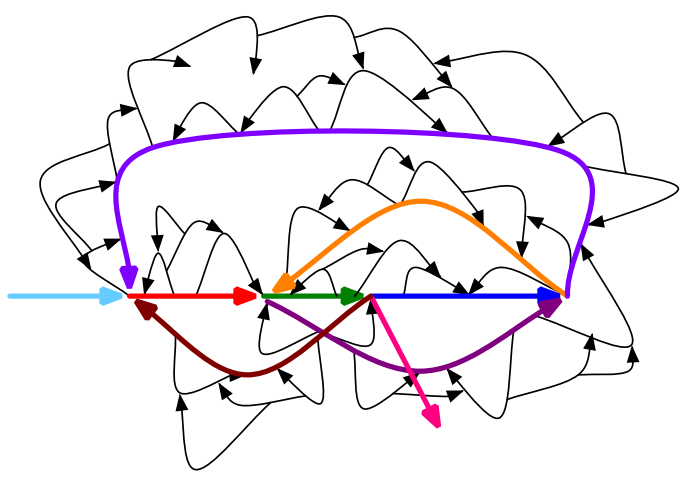
\includegraphics[width=0.5\textwidth]{poglavlja/3/slike/eksplozija-baloncica.png}
	\caption{Eksplozija balon\v ci\'ca.}
	\label{slika:eksplozija baloncica}
\end{figure}

\section{Zadaci sa vežbi}
\setexamplecodestyle

U nastavku će biti predstavljeni zadaci sa vežbi na kursu rađeni u programskom jeziku Python.

\subsection{Maximal Non Branching Path}

\lstinputlisting[language=Python]{poglavlja/3/kodovi/1.py}

\subsection{All Euler Cycles}

\lstinputlisting[language=Python]{poglavlja/3/kodovi/2.py}

\subsection{String Spelled By Gapped Patterns}

\lstinputlisting[language=Python]{poglavlja/3/kodovi/3.py}

\blankpage